\chapter{Implemented changes}\label{jiveImpl}%hva ble gjort, hvordan bruke funksjonene. Ikke så mye om hvordan. begrunne prioriteter?

This chapter will list the changes that were made to \gls{jive}, and give some information on how they work.

In order to be able to implement any changes, it was first necessary to gain some knowledge about how Eclipse's plugin-framework is used, and how \gls{jive} is structured.
The graphical components of \gls{jive} utilize the \gls{gef}, an \gls{mvc} framework used to create graphical views and editors in Eclipse.

%identifisering av instansierte grensesnitt, lambdaer og abstrakte klaser
\section{Labeling of objects}\label{implLabel}

The first change to be implemented was the identification and presentation of instantiated interfaces.
These are now displayed in the diagrams with an appropriate icon, as well as being labeled with the interface they implement, instead of the generic class name that they are assigned by default.
An example of this is shown in \cref{fig:JiveNewIcon}.
This function was also expanded to identify and label instances of abstract classes, and the \glspl{lambdaExpression} that were introduced with Java 8.
In order to still allow the actual class name to be visible, the tool-tip shown when hovering the mouse pointer over an object remains unmodified, and displays the actual class name and icon.
\begin{figure}[H]
	\centering
	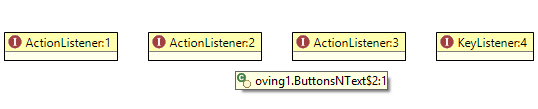
\includegraphics[width=\textwidth]{UIJiveInterfaceIcon}
	\caption[A view of how instantiated interfaces are shown after the modification.]{A view of how instantiated interfaces are shown after the modification. Also shown is the tool-tip text for the second instance from the left. Originally, they would be labeled as `ButtonsNText\$1:1', `ButtonsNText\$2:1' and so on, with the green class-icon.}
	\label{fig:JiveNewIcon}
\end{figure}

%utvidelse av filteret
\section{Expanding the filter}\label{implFilter}

The filtering function was expanded with the ability to specify packages that are not to be excluded from the execution model, as suggested in \cref{jiveSuggestions}.
Adding a package for inclusion is done by prefixing the package-name with a `+' when adding it to the filter, as shown in \cref{fig:UIJiveLaunchConfigDefaultFilter+swing}.
As an example, the default filter excludes the `javax' package, and any subpackages that are not specifically listed with a `+' in front.
When adding the line `+javax.swing.*' in order to let Swing--components through the filter, every subpackage of `javax.swing' is let though the filter as well, which is the intended design.

\begin{figure}[H]
	\centering
	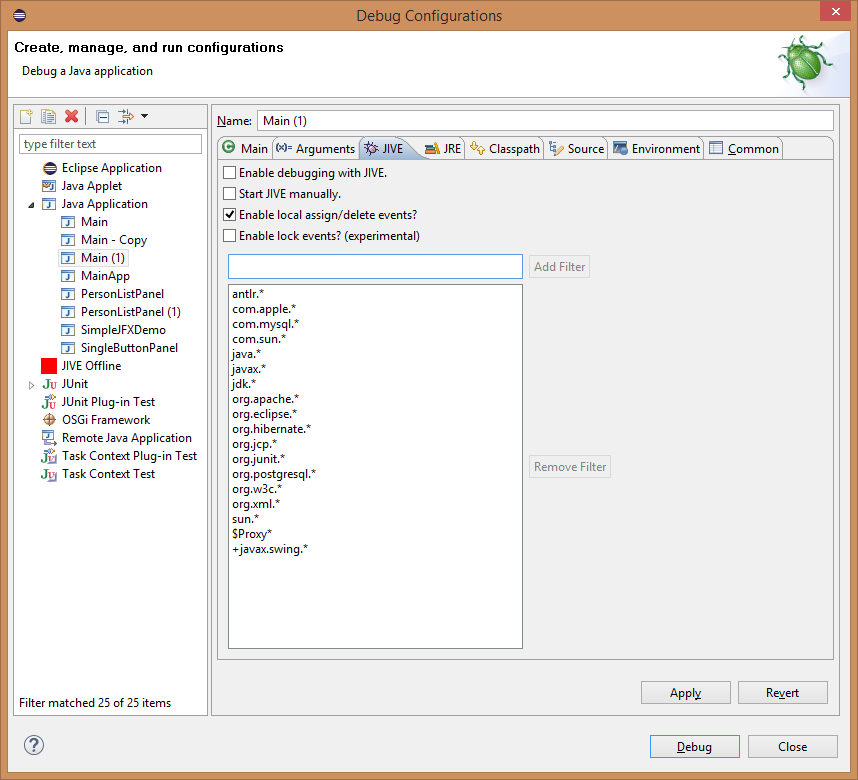
\includegraphics[width=\textwidth]{UIJiveLaunchConfigDefaultFilter+swing}
	\caption[The JIVE-tab in the launch configuration menu.]{The JIVE-tab in the launch configuration menu, showing the default exclusion filter, with the addition of an entry to include `javax.swing.*'.}
	\label{fig:UIJiveLaunchConfigDefaultFilter+swing}
\end{figure}

Unfortunately, there are a lot of classes in both Swing and its subpackages that are not used directly when writing Swing-programs, and a user will have no interest in seeing these in the diagrams.
This can result in very poor performance -- as unnecessary events are logged and added to the underlying model -- as well as cluttered diagrams.
By adding these unwanted classes to the filter for exclusion, the problem is handled.
Depending on the package in question, the amount of extra items added to the filter can become quite large, and identifying all unwanted classes and subpackages may take hours at worst.
A weakness in the filter is related to the problem of unwanted packages.
Due to its design, allowing the contents of a package will also allow any classes that are contained directly within the parent package, as the parent also has to be removed from the internal list of exclusions that make up the filter.
This is not a big problem in the case of `javax.swing', as the `javax' package does not contain any classes, but there are most likely other packages that will show this behavior.

Internally, the filter is still only excluding events.
The changes were made to the construction-phase, where every package that is found in the Eclipse workspace is added if it is found in the list that the user has made.
This allows the removal of entries that are marked with a `+', but results in a rather large filter that affects the performance negatively, as is shown in the evaluation results in \cref{jiveEvalPerf}.
During development, the performance was not a major concern, and as such, it was not prioritized.
It is possible to reduce the impact of the filtering changes by further altering the construction process to result in a smaller filter.
By improving the way an event is checked against the filter, possibly by looking up hashed values instead of comparing strings, further gains should be possible.


%isolert visning av sekvens
\section{The isolated view}\label{isoView}

The isolated view was implemented as a separate view-tab, and does what was proposed in \cref{fig:seqOving4IsolatedMock}: It displays the events caused by the selected event, and hides everything else.
\Cref{fig:MMI-oving4-SeqIsoDiag-AWT-Event-Thread} shows what \cref{fig:seqOving4IsolatedMock} looked like after the modification.
\Cref{fig:MMI-oving4-SeqIsoDiag-valueChanged} shows a similar, but slightly more complex situation in the isolated view.
By right-clicking on an event in the regular sequence-diagram, and selecting the \emph{Isolated view}-option, shown in \cref{fig:UISeqRightClickNew}, the isolated view is triggered.
It is also possible to further focus on a part of the diagram from within the isolated view, by right-clicking on the desired event, and selecting the \emph{Isolated view}-option again.
All of the functionality from the regular sequence-diagram has been retained in the isolated view, so that the only difference is which parts of the execution are visible.
\begin{figure}[H]
	\centering
	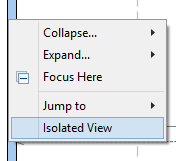
\includegraphics{UIseqRightClickNew}
	\caption{The new \emph{Isolated view} option.}
	\label{fig:UISeqRightClickNew}
\end{figure}

\begin{figure}[H]
	\centering
	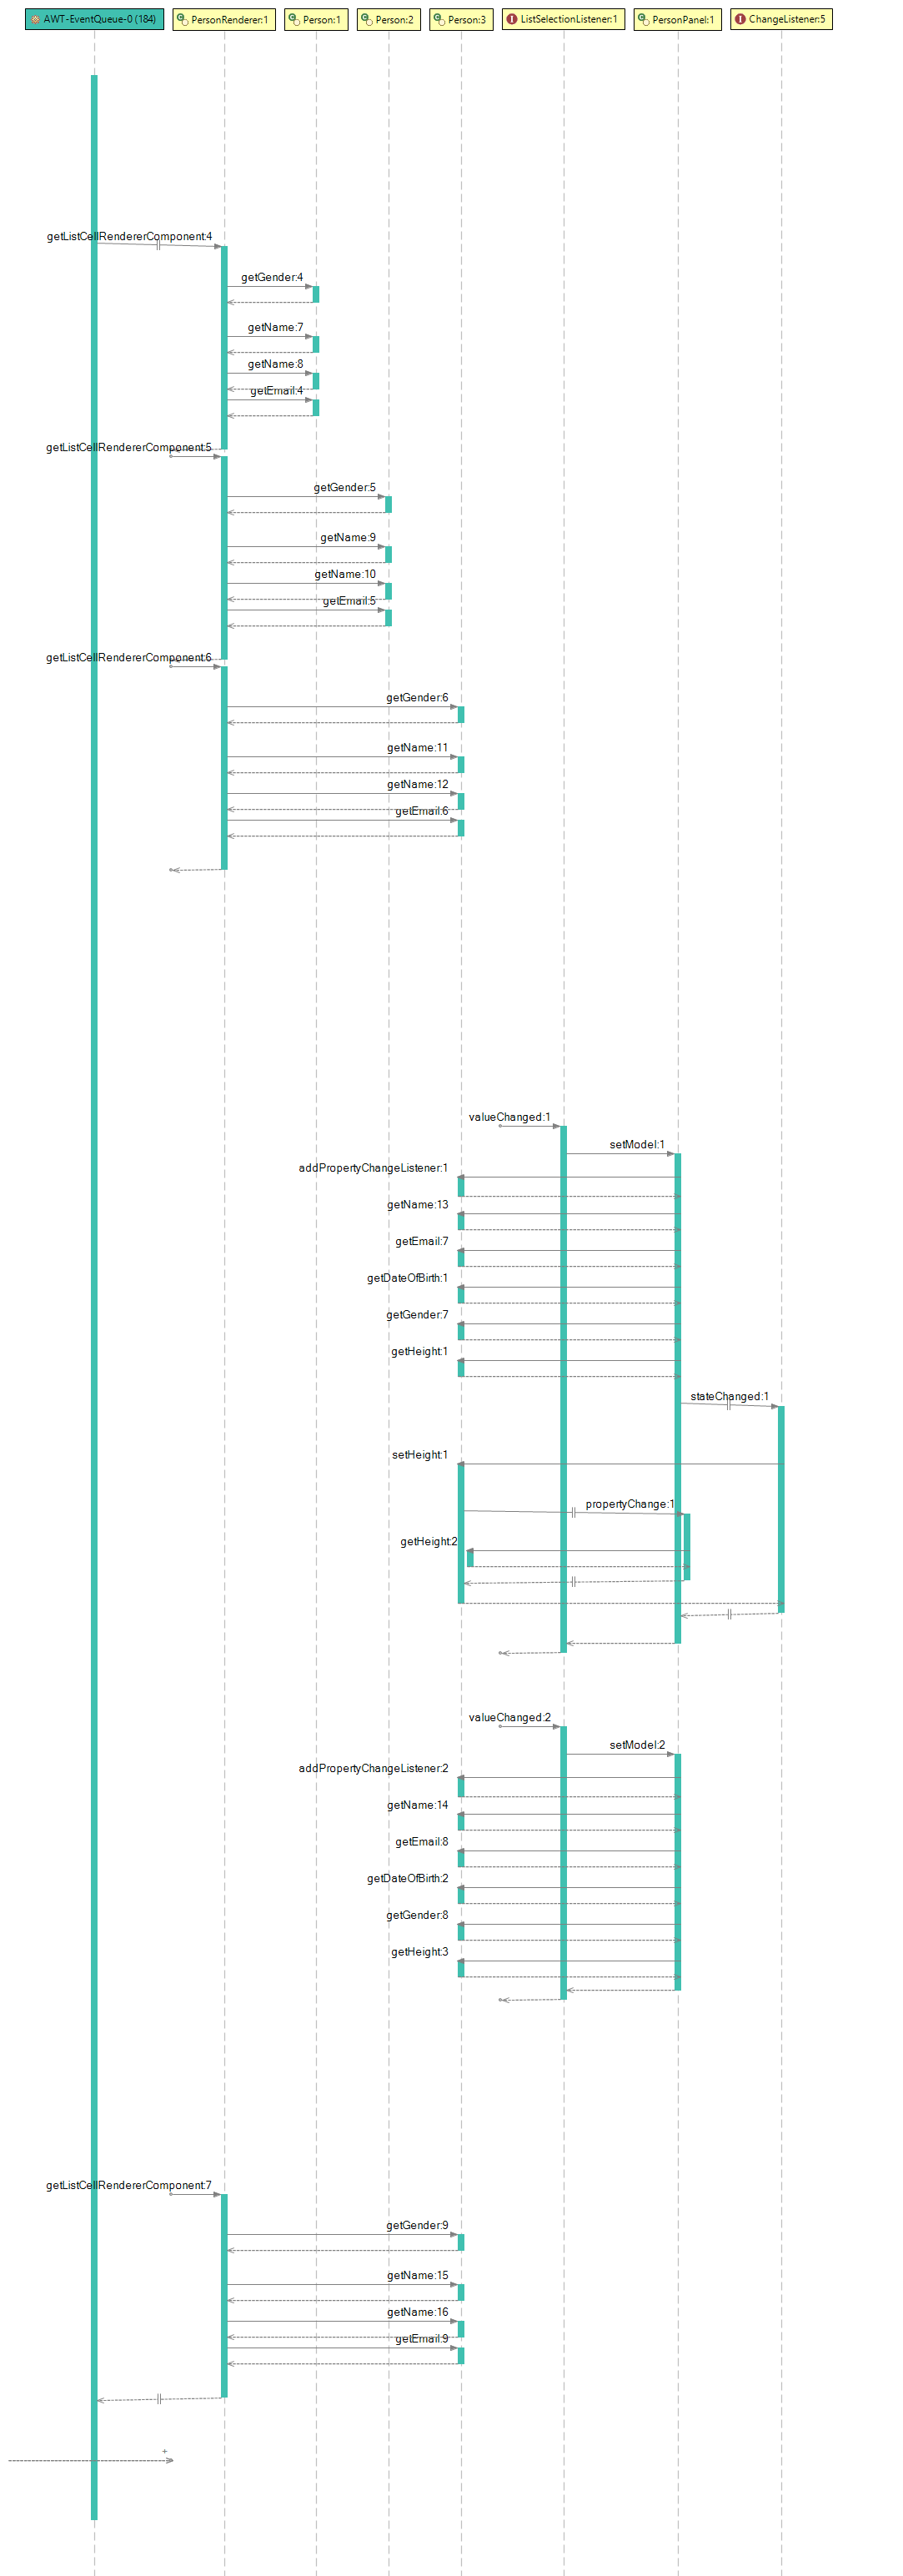
\includegraphics[width=\textwidth, trim= 0cm 50cm 0cm 0cm, clip]{MMI-oving4-SeqIsoDiag-AWT-Event-Thread}
	\caption[How \cref{fig:seqOving4CrossLines} looks in the isolated view.]{How \cref{fig:seqOving4CrossLines} looks in the isolated view. The three last elements shown on the top are referred to in parts of the diagram not shown. This view was achieved by initiating the isolated view from the `AWT-EventQueue' lifeline.}
	\label{fig:MMI-oving4-SeqIsoDiag-AWT-Event-Thread}
\end{figure}

\begin{figure}[H]
	\centering
	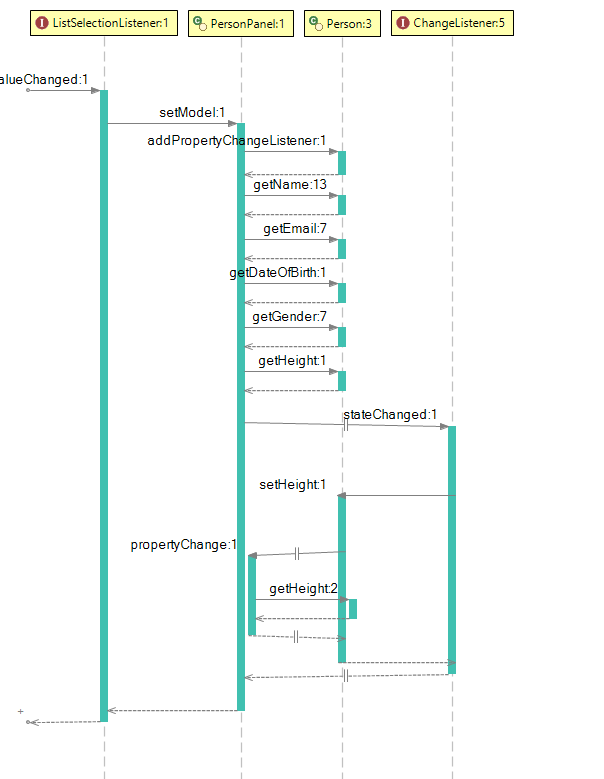
\includegraphics[width=\textwidth, trim= 0cm 0cm 0cm 0cm, clip]{MMI-oving4-SeqIsoDiag-valueChanged}
	\caption{Another example of the isolated view, showing a significantly reorganized diagram.}
	\label{fig:MMI-oving4-SeqIsoDiag-valueChanged}
\end{figure}

%mer avslappede søkekrav - er ikke utført for alle typer søk, er det verd å nevne i det hele tatt?
\section{Relaxing the search}\label{implSearch}
The searching functionality was relaxed by allowing partial matches, and disabling case sensitivity.
While relaxing the search may cause false positives, a user should be able to identify such cases quickly, or at least identify the results they were looking for.
The fact that partial matches and case insensitivity is the standard behavior in most search-engines, sets an expectation for the behavior of the search within \gls{jive}.
Unfortunately, due to the existing implementation consisting of separate searching- and matching-methods for each search type, not all searches were updated to this relaxed state in order to prioritize more important changes.
The only changed search was the \emph{Object created}-search.
Ideally the searches should all be matched through the same matching method, only differing in the gathering of necessary information.

